%
Germanium can be enriched in the \bb\ isotope \Ge{76}and transformed into high-purity germanium (HPGe) detectors, devices characterized by superb energy resolution and high efficiency. 

HPGe detectors have a long-standing record in neutrinoless double beta decay searches, going back to the late 1960s \cite{Fiorini:1967in,Fiorini:1970}. In the 1990s, the two most sensitive experiments used this technology: \textsc{Heidelberg-Moscow} (HM) ran in the Laboratori Nazionali del Gran Sasso (LNGS) and set a lower limit on the \bbonu\ half-life of \Ge{76} of $1.9 \times 10^{25}$~years (90\% CL) \cite{Klapdor-Kleingrothaus:2000eir}. However, a subset of the HM collaboration published a controversial claim of evidence for \bbonu\ decay \cite{Klapdor-Kleingrothaus:2001oba, Klapdor-Kleingrothaus:2006zcr}, which sparked at the time an intense debate in the community (see, for example, ref.~\cite{Aalseth:2002dt}). The International Germanium Experiment (IGEX) operated in the Homestake Mine (USA), the ---at the time very small--- Canfranc Underground Laboratory (Spain) and the Baksan Neutrino Observatory (Russia), setting a slightly worse limit than HM, $T^{0\nu}_{1/2}(\Ge{76}) \geq 1.6 \times 10^{25}$~years (90\% CL) \cite{IGEX:2002bce}. Those negative results, however, were not sufficiently precise to discard the claim of evidence put forward in \cite{Klapdor-Kleingrothaus:2001oba, Klapdor-Kleingrothaus:2006zcr}, which reminded an open question for many years. 

HM and IGEX were succeeded by two new experiments, the GERmanium Detector Array (GERDA) \cite{GERDA:2020xhi} and the \textsc{Majorana Demonstrator} \cite{Majorana:2022udl}, which employed novel types of HPGe devices with improved energy resolution and pulse-shape identification which provided detailed information about the topology of events through the time structure of the recorded charge signal.

GERDA, located at LNGS, operated bare HPGe detectors in a high-purity instrumented liquid argon (LAr) cryostat, which provided not only the cooling for the HPGe devices, but also served as active shielding and veto against external and internal background events. With a background index of $5.2\times10^{-4}$~\ckky\ and an energy resolution of $\sim3$~keV (FWHM) at $Q_{\bb}=2039$~keV \cite{GERDA:2020xhi}, GERDA has been the first \bbonu-decay experiment to operate in the ``background-free regime'' (i.e., less than one expected background count in the signal window). With a total published exposure of 127.2~kg~yr, the derived lower limit on the \bbonu\ half-life of \Ge{76} is $1.8\times10^{26}$~yr (90\% C.L.) \cite{GERDA:2020xhi}. 

The \textsc{Majorana Demonstrator} operated its HPGe detectors at the Sanford Underground Research Facility (SURF) in a high-purity shield built with electro-formed copper produced deep underground. With a world-leading energy resolution of 2.52~keV FWHM at \Qbb\ and after accumulating an exposure of 64.5~kg~yr, the experiment set a half-life lower limit of $8.3\times10^{25}$~yr (90\% CL) \cite{Majorana:2022udl}.

Building on the success of GERDA and the \textsc{Majorana Demonstrator}, the LEGEND \cite{LEGEND:2021bnm} collaboration is developing a staged \bbonu-decay experimental program aiming at an ultimate sensitivity to the \Ge{76} half-life beyond $10^{28}$~years. 
LEGEND will make use of new inverted-coaxial point-contact (ICPC) HPGe detectors with exceptional energy resolution (0.12\% FWHM at 2039~keV) and more than a factor of two greater mass per crystal over previous experiments. As done in GERDA, the HPGe detectors will be operated immersed in LAr.

%%%%%
\begin{figure}[t!b!]
\begin{center}
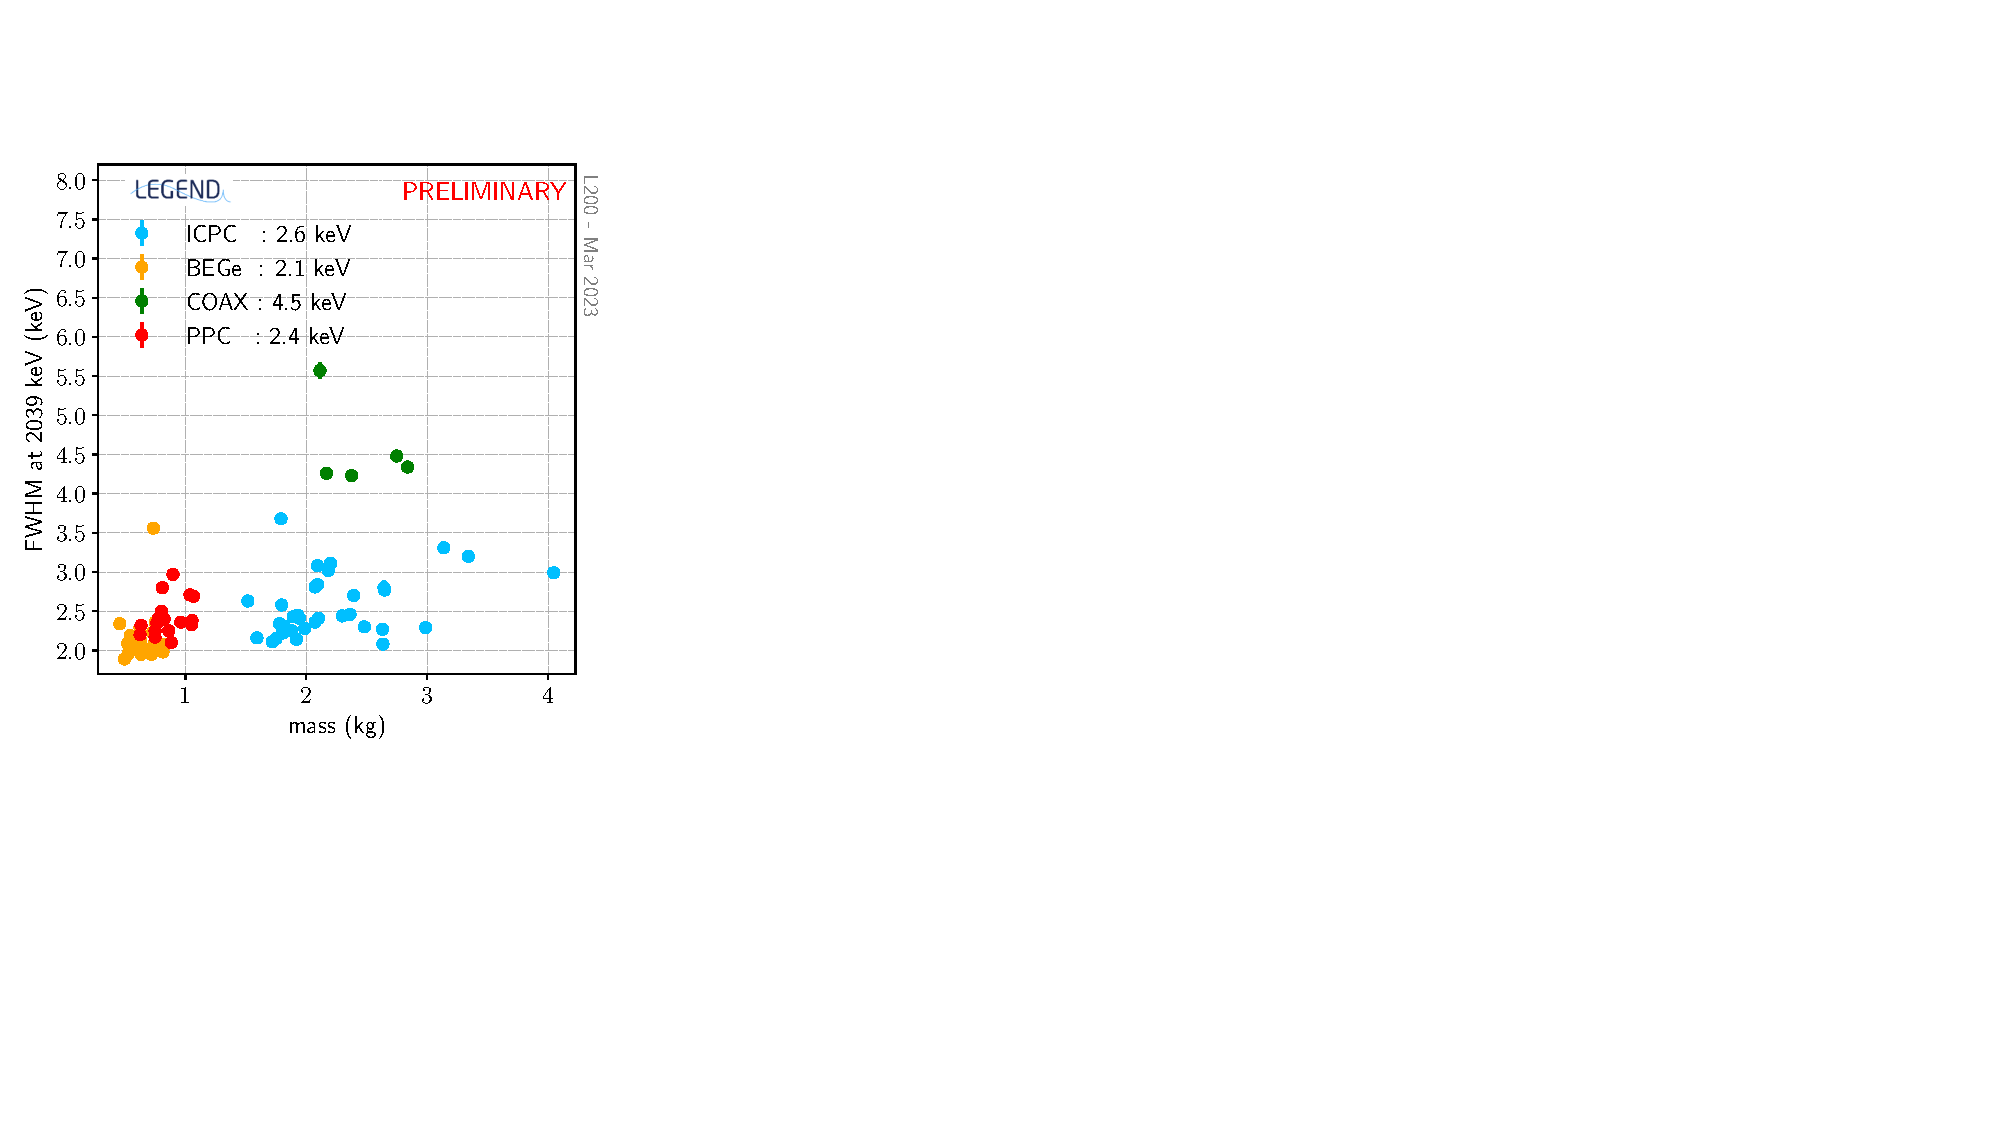
\includegraphics[width=0.55\textwidth]{img/legend-200.pdf}
\end{center}
\caption{Preliminary FWHM energy resolution at the \Ge{76} Q-value for the $\sim$100 HPGe detectors currently deployed in LEGEND-200. The different colors indicate different HPGe detector types.}  \label{fig:legend-200}
\end{figure}
%%%%%

LEGEND-200, the first phase of the experiment, is operating 200~kg of germanium detectors ---\thinspace the existing 70 kg of enriched detectors from the \textsc{Majorana Demonstrator} and GERDA, plus an additional 130~kg of newly produced ICPC detectors\thinspace--- in an upgrade of the GERDA infrastructures at LNGS incorporating technologies from the \textsc{Majorana Demonstrator}. First LEGEND-200 results related to its outstanding energy resolution are shown in Fig.~\ref{fig:legend-200}. A reduction by a factor of 2.5 with respect to the GERDA background rate is expected, aiming at a sensitivity to the \bbonu\ half-life of about $10^{27}$~yr for  an exposure of 1 ton~yr. The second phase of the experiment, LEGEND-1000, has a background goal of less than $10^{-5}$~\ckky, a 20-fold reduction with respect to LEGEND-200 expected to come from the use of underground-sourced argon (which does not contain the radioactive isotopes $^{42}$Ar and its daughter $^{42}$K), improvements in the radiopurity of materials and the exclusive use of ICPC HPGe detectors.
